\def\QRCODE{MASTER_mispa_TUT.IMG.lbp_matlabqrcode.png}
\def\QRPAGE{http://www.iptutorials.science/tree/master/MASTER_mispa/TUT.IMG.lbp/matlab}
\mcorrectionsection{Matlab correction}

\subsection{LBP computation}
Each pixel is given a specific 8 bits value according to a code as follows. The parfor loop is used for speed.

\begin{matlab}
% binary code for pixel description
code = [1 2 4; 8 0 16; 32 64 128];

% loop over all pixels
parfor i=2:m-1
    for j=2:n-1
        w = A(i-1:i+1,j-1:j+1);
        w = (w >= A(i,j));
        w = w.*code;
        B(i,j) = sum(w(:));
    end
end
\end{matlab}

Then, all values (except for border values) are symmarized in the histogram.

\begin{matlab}
B = B(2:end-1,2:end-1);
h = histcounts(B(:), 256, 'normalization', 'probability');
\end{matlab}

For the first image of sand, the histogram is shown in Fig.\ref{fig:lbp:matlab:lbpsand1}.

\begin{figure}[htbp]
 \centering
 
 \subfloat[Texture image.]{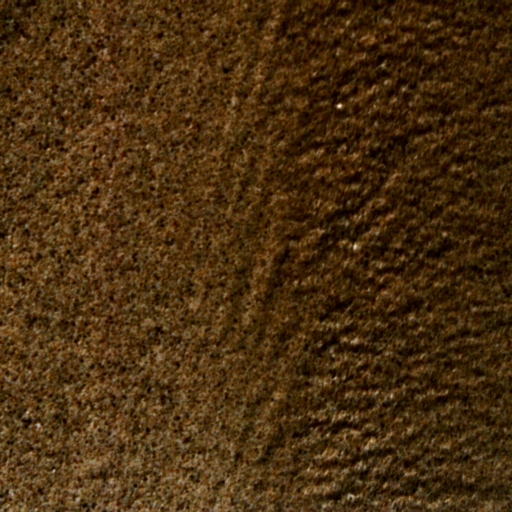
\includegraphics[width=.4\linewidth]{Sand.1.png}}\hfill
 \subfloat[LBP of texture.]{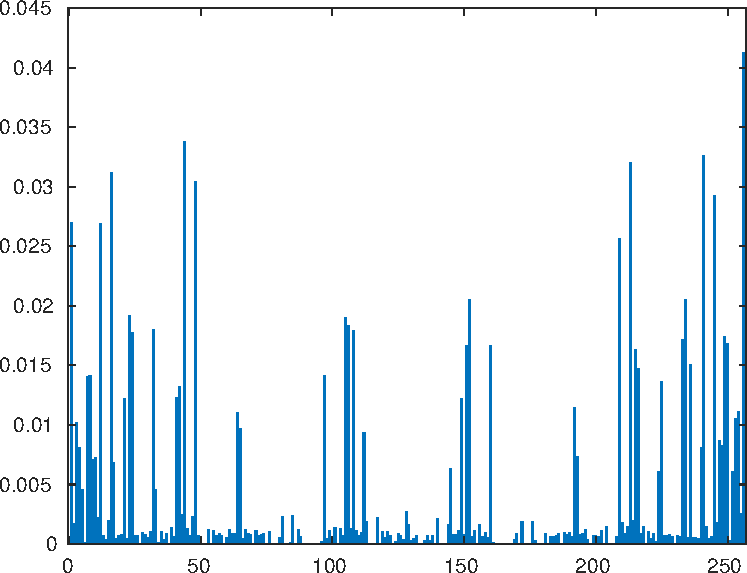
\includegraphics[width=.55\linewidth]{sand1_lbp.pdf}}
 
 \caption{Illustration of the Local Binary Pattern computed on an entire image.}
 \label{fig:lbp:matlab:lbpsand1}
\end{figure}

\subsection{Classification}
For all images of the same family, the LBP are computed and represented in the same graph. The histograms really look similar (see Fig.\ref{fig:lbp:matlab:lbp}). The following code is used for the ``sand'' family.

\begin{matlab}
rep='images/';
name_image = 'Sand';
LBP_Sand = cell(1,4);

for i = 1:4
    A = imread(strcat(rep, name_image,'.',num2str(i),'.bmp'));
    A = rgb2gray(A);
    LBP_Sand{i} = LBP(A);
end

figure;
hold on;
corange = {[1 0 0],[1 0.2 0], [1 0.4 0], [1 0.6 0]};
for i=1:4
    plot(LBP_Sand{i},'color',corange{i});
end
\end{matlab}

\begin{figure}[htbp]
 \centering
 
 \subfloat[Metal image example.]{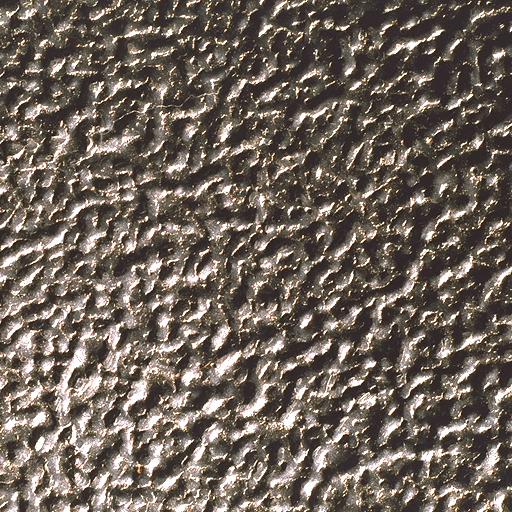
\includegraphics[width=.3\linewidth]{Metal.1.png}}\hfill
 \subfloat[Sand image example.]{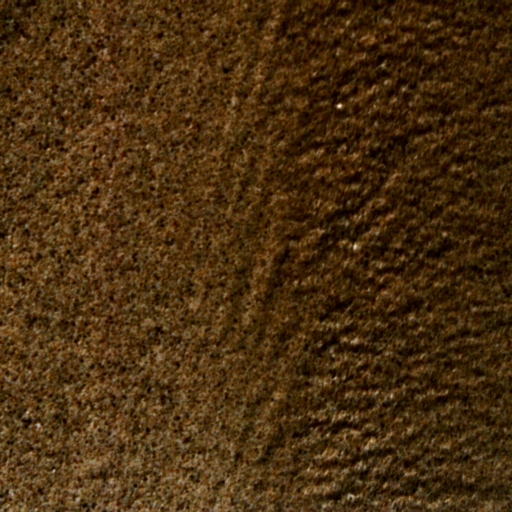
\includegraphics[width=.3\linewidth]{Sand.1.png}}\hfill
\subfloat[Terrain image example.]{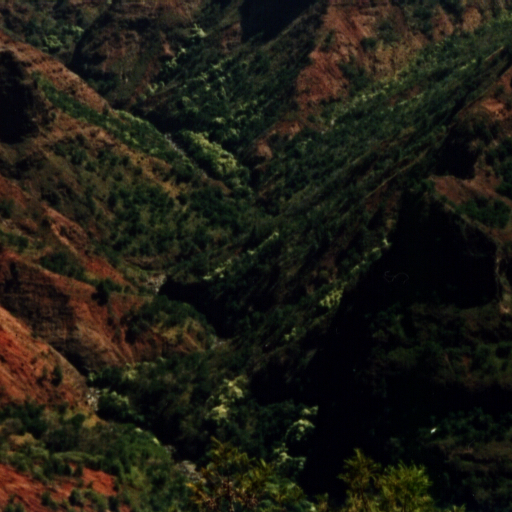
\includegraphics[width=.3\linewidth]{Terrain.1.png}}

 \subfloat[Four metal images.]{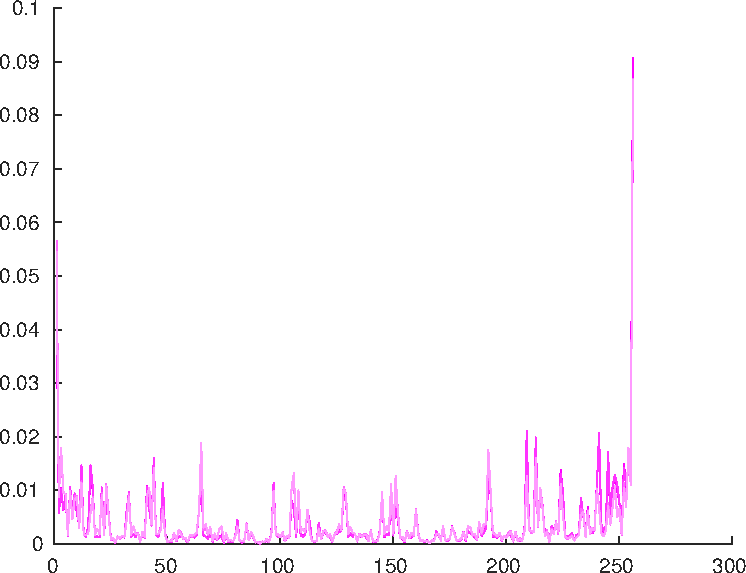
\includegraphics[width=.3\linewidth]{metal_lbp.pdf}}\hfill
 \subfloat[Four sand images.]{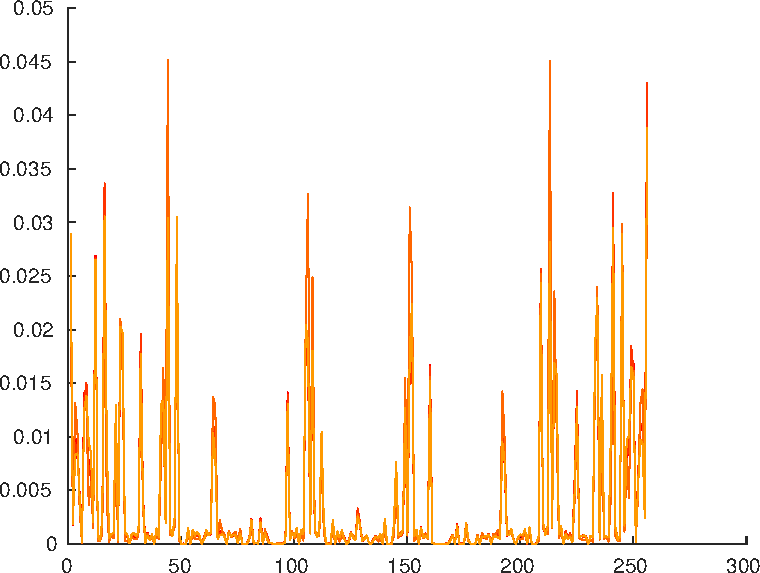
\includegraphics[width=.3\linewidth]{sand_lbp.pdf}}\hfill
\subfloat[Four terrain images.]{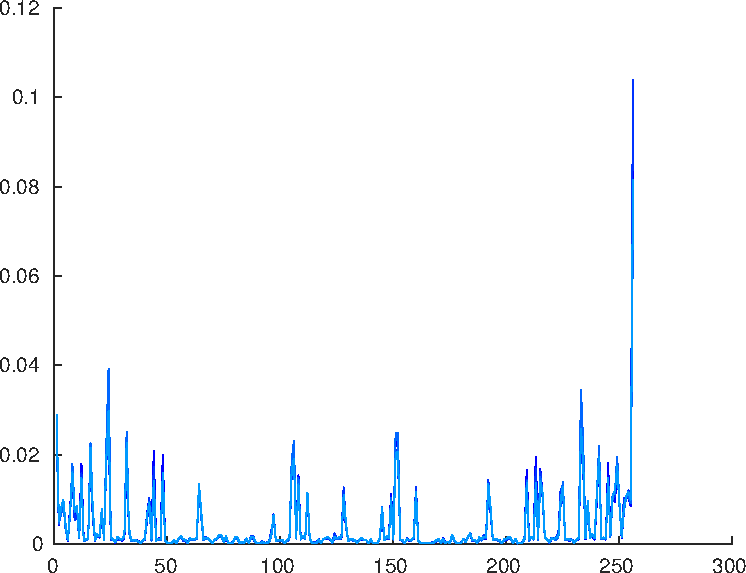
\includegraphics[width=.3\linewidth]{terrain_lbp.pdf}}
 \caption{Illustration of the LBP of 4 images of each family. The histogram are almost equivalent, which shows that this descriptor can be employed to discriminate between the different families.}
 \label{fig:lbp:matlab:lbp}
\end{figure}

A distance criterion is used to compare the different histograms: the classical SAD (Sum of Absolute Differences) gives a numerical values. All pairs of distances are concatenated in a matrix, displayed as an image in Fig.\ref{fig:lbp:matlab:dists}.

\begin{matlab}
LBP = [LBP_Terrain,LBP_Metal,LBP_Sand];
dist = zeros(12,12);
parfor i=1:12
    X(i,:) = LBP{i}';% for later K-means computation
    for j=1:12
        dist(i,j) = sum(abs(LBP{i}-LBP{j}));
    end
end

figure;
imagesc(dist);
colormap('gray');
\end{matlab}


\begin{figure}[htbp]
 \centering
 
 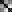
\includegraphics[width=.4\linewidth]{sad_lbp.png}

 
 \caption{Sum of Absolute Differences between the different LBP histograms of each image. 3 families of 4 textures are represented here, terrain images are in the first part, metal images in the second and sand images in the last. Black represents 0  distance and white is 1 (highest distance, the values are normalized).}
 \label{fig:lbp:matlab:dists}
\end{figure}

The kmeans algorithm uses such a distance, and we can verify that the clustering process works as expected. The result is presented in the next box.
\begin{matlab}
 % labels 1-4, 5-8, 9-12 should be equal, respectively
label = kmeans(X,3,'replicates',5)'
\end{matlab}

\begin{mwindow}
% the 3 families are well classified
label =   3   3   3   3   2   2   2   2   1   1   1   1
\end{mwindow}


